\documentclass[10pt]{article}
\usepackage[margin=0.5cm,paperwidth=15cm,paperheight=10cm]{geometry}
\usepackage{tikz}
\usetikzlibrary{positioning,arrows.meta,calc}
\pagestyle{empty}

\begin{document}
\begin{center}
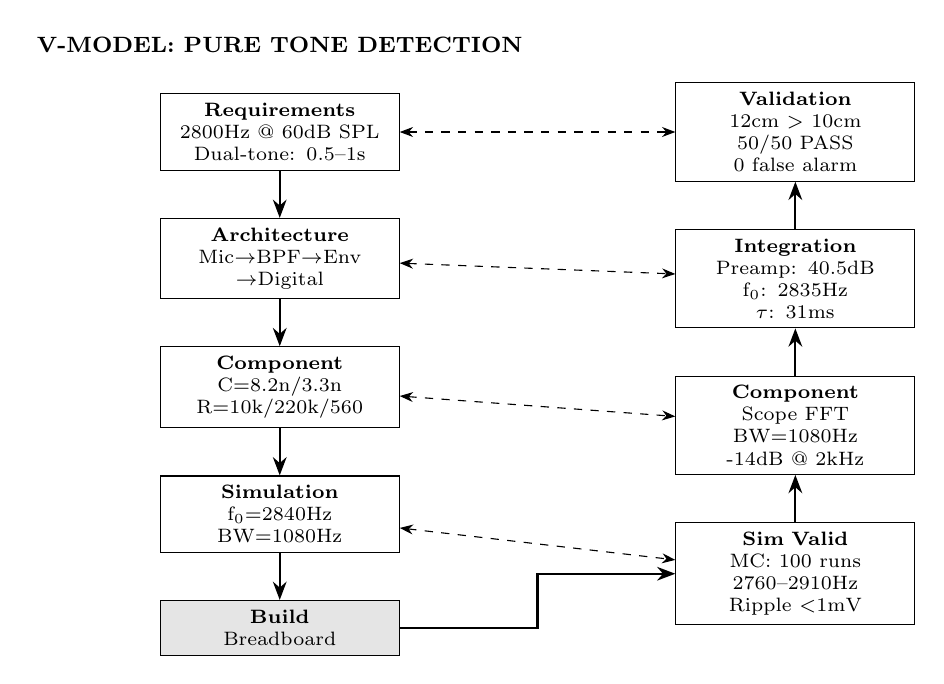
\begin{tikzpicture}[
  node distance=0.6cm and 1.2cm,
  box/.style={rectangle, draw, text width=2.8cm, align=center, font=\scriptsize, minimum height=0.7cm},
  arrow/.style={->, >=Stealth, thick},
  dasharrow/.style={<->, >=Stealth, dashed}
]

% Title
\node[font=\footnotesize\bfseries] (title) {V-MODEL: PURE TONE DETECTION};

% Left side (Design)
\node[box, below=0.4cm of title] (req) {\textbf{Requirements}\\2800Hz @ 60dB SPL\\Dual-tone: 0.5--1s};
\node[box, below=of req] (arch) {\textbf{Architecture}\\Mic$\rightarrow$BPF$\rightarrow$Env\\$\rightarrow$Digital};
\node[box, below=of arch] (comp) {\textbf{Component}\\C=8.2n/3.3n\\R=10k/220k/560};
\node[box, below=of comp] (sim) {\textbf{Simulation}\\f$_0$=2840Hz\\BW=1080Hz};

% Bottom (Implementation)
\node[box, below=of sim, fill=gray!20] (impl) {\textbf{Build}\\Breadboard};

% Right side (Validation)
\node[box, right=3.5cm of req] (sysval) {\textbf{Validation}\\12cm $>$ 10cm\\50/50 PASS\\0 false alarm};
\node[box, below=of sysval] (inttest) {\textbf{Integration}\\Preamp: 40.5dB\\f$_0$: 2835Hz\\$\tau$: 31ms};
\node[box, below=of inttest] (comptest) {\textbf{Component}\\Scope FFT\\BW=1080Hz\\-14dB @ 2kHz};
\node[box, below=of comptest] (simval) {\textbf{Sim Valid}\\MC: 100 runs\\2760--2910Hz\\Ripple $<$1mV};

% Arrows - Left descending
\draw[arrow] (req) -- (arch);
\draw[arrow] (arch) -- (comp);
\draw[arrow] (comp) -- (sim);
\draw[arrow] (sim) -- (impl);

% Arrows - Right ascending
\draw[arrow] (impl) -| ($(impl)!0.5!(simval)$) |- (simval);
\draw[arrow] (simval) -- (comptest);
\draw[arrow] (comptest) -- (inttest);
\draw[arrow] (inttest) -- (sysval);

% Horizontal validation arrows
\draw[dasharrow] (req) -- (sysval);
\draw[dasharrow] (arch) -- (inttest);
\draw[dasharrow] (comp) -- (comptest);
\draw[dasharrow] (sim) -- (simval);

\end{tikzpicture}
\end{center}
\end{document}
